\subsection{Perfect Sets and the Cantor Set}

\begin{theorem} \label{thm:nonempty-perfect-subset-rk-uncountable} \hlt{Euclidean Perfect Sets Are Uncountable}\\
Let $k\in\N$, and let $\emptyset\neq P\subseteq\R^k$ be perfect. Then $P$ is uncountable.
\begin{proof}
\begin{enumerate}[label=(\roman*)]
\setlength{\itemsep}{0pt}
\item \hlt{Enumeration}: Suppose $P$ is at most countable.\\
By Proposition \ref{prop:at-most-countable-iff-enumerable-image}, choose $(\mathbf{x}_n)$ satisfying $P=\{\mathbf{x}_n:n\in\N\}$. Set $\mathbf{c}_1\defeq\mathbf{x}_1$ and $r_1\defeq1$.
\item \hlt{Recursive construction}: Suppose $\mathbf{c}_n\in P$ and $r_n>0$ have been defined.\\
The point $\mathbf{c}_n$ belongs to $P^{\operatorname{acc}}$ by Definition \ref{def:bounded-and-perfect-metric-sets}(ii). The ball $B_{r_n}(\mathbf{c}_n)$ is a neighborhood of $\mathbf{c}_n$ by Theorem \ref{thm:every-neighborhood-open}.\\
Hence $P\cap B_{r_n}(\mathbf{c}_n)$ is infinite by Theorem \ref{thm:limit-point-neighborhoods-infinitely-many}. Set $A_n\defeq\{j\in\N:\mathbf{x}_j\in B_{r_n}(\mathbf{c}_n),\ \mathbf{x}_j\neq\mathbf{x}_n\}\neq\emptyset$.\\
The minimum $m_n\defeq\min A_n$ exists by Assumption \ref{assump:well-ordering-positive-integers}. Put $\mathbf{y}_n\defeq\mathbf{x}_{m_n}$ and $\mathbf{c}_{n+1}\defeq\mathbf{y}_n$.\\
Set $\delta_n\defeq\min\{r_n-\norm{\mathbf{y}_n-\mathbf{c}_n}_2,\norm{\mathbf{y}_n-\mathbf{x}_n}_2\}$ and $r_{n+1}\defeq\frac{\delta_n}{2}$.\\
The relations $\norm{\mathbf{y}_n-\mathbf{c}_n}_2<r_n$ and $\norm{\mathbf{y}_n-\mathbf{x}_n}_2>0$ imply $\delta_n>0$ and $r_{n+1}>0$.
\item \hlt{Containment and avoidance}: Fix $\mathbf{u}\in\overline{B}_{r_{n+1}}(\mathbf{c}_{n+1})$.\\
Then $\norm{\mathbf{u}-\mathbf{c}_n}_2\leq r_{n+1}+\norm{\mathbf{y}_n-\mathbf{c}_n}_2\leq\frac{r_n+\norm{\mathbf{y}_n-\mathbf{c}_n}_2}{2}<r_n$ by the triangle inequality.\\
Thus $\overline{B}_{r_{n+1}}(\mathbf{c}_{n+1})\subseteq B_{r_n}(\mathbf{c}_n)$. Hence $\norm{\mathbf{x}_n-\mathbf{c}_{n+1}}_2=\norm{\mathbf{x}_n-\mathbf{y}_n}_2\geq\delta_n=2r_{n+1}>r_{n+1}$, so $\mathbf{x}_n\notin\overline{B}_{r_{n+1}}(\mathbf{c}_{n+1})$.
\item \hlt{Compact intersection}: Put $K_n\defeq\overline{B}_{r_n}(\mathbf{c}_n)\cap P$; then $\mathbf{c}_n\in K_n$.\\
The set $P$ is closed by Definition \ref{def:bounded-and-perfect-metric-sets}(ii). The ball $\overline{B}_{r_n}(\mathbf{c}_n)$ is closed by Corollary \ref{cor:closed-balls-are-closed}.\\
Set $K_n$ is closed by Theorem \ref{thm:metric-open-closed-set-calculus}(ii) and bounded. Hence $K_n$ is compact by Theorem \ref{thm:heine-borel-rk}, direction $(i)\Rightarrow(ii)$.\\
The inclusion $K_{n+1}\subseteq K_n$ holds by stage (iii). Choose $\mathbf{z}\in\bigcap\limits_{n=1}^{\infty}K_n$ by Corollary \ref{cor:nested-nonempty-compact-intersection}.\\
Then $\mathbf{z}\in K_1\subseteq P$ and $(\forall n\in\N)\,[\mathbf{z}\in K_{n+1}\land\mathbf{x}_n\notin K_{n+1}]$, so $(\forall n\in\N)\,\mathbf{z}\neq\mathbf{x}_n$.\\
This contradicts $P=\{\mathbf{x}_n:n\in\N\}$. Hence $P$ is uncountable by Definition \ref{def:finite-countable-uncountable}(iv)--(v).
\end{enumerate}
\hlt{Structural Commentary}: The enumeration determines nested compact balls whose $n$th refinement excludes $\mathbf{x}_n$.\\
\hlt{Key Insight}: Perfectness selects centers; compactness preserves one point through every exclusion.
\end{proof}
\end{theorem}

Figure \ref{fig:perfect-set-nested-interval-avoidance} depicts stage (iii) on the real line.
\begin{illustrationfigure}[H]
  \centering
  \begin{tikzpicture}[
  every node/.style={font=\small},
  axis/.style={gray!65, line width=0.55pt},
  interval/.style={blue!70!black, line width=1.35pt},
  smallinterval/.style={orange!80!black, line width=1.45pt},
  guide/.style={gray!55, dashed, line width=0.45pt},
  point/.style={circle, fill=black, inner sep=1.45pt}
]
  \draw[axis] (-0.25,0) -- (7.25,0);

  \coordinate (iOneL) at (0.45,0);
  \coordinate (iOneR) at (6.85,0);
  \coordinate (xone) at (2.45,0);
  \coordinate (iTwoL) at (4.35,0);
  \coordinate (ytwo) at (5.05,0);
  \coordinate (iTwoR) at (5.85,0);

  \draw[interval] ($(iOneL)+(0,0.62)$) -- ($(iOneR)+(0,0.62)$);
  \draw[interval] ($(iOneL)+(0,0.34)$) -- ($(iOneL)+(0,0.90)$);
  \draw[interval] ($(iOneR)+(0,0.34)$) -- ($(iOneR)+(0,0.90)$);
  \node[blue!70!black, above] at (3.65,0.92) {$I_1$};

  \draw[smallinterval] ($(iTwoL)+(0,-0.50)$) -- ($(iTwoR)+(0,-0.50)$);
  \draw[smallinterval] ($(iTwoL)+(0,-0.76)$) -- ($(iTwoL)+(0,-0.24)$);
  \draw[smallinterval] ($(iTwoR)+(0,-0.76)$) -- ($(iTwoR)+(0,-0.24)$);
  \node[orange!80!black, below] at ($(ytwo)+(0,-0.78)$) {$I_2$};

  \draw[guide] (iTwoL) -- ($(iTwoL)+(0,-0.50)$);
  \draw[guide] (iTwoR) -- ($(iTwoR)+(0,-0.50)$);

  \node[point] at (xone) {};
  \node[below] at (xone) {$x_1$};

  \node[point] at (ytwo) {};
  \node[above] at (ytwo) {$y_2\in P$};

  \node[gray!65] at (3.40,-0.50) {$x_1\notin I_2$};
\end{tikzpicture}

  \caption{A closed interval $I_2\subseteq I_1$ centered at $y_1\in P$ avoids $x_1$.}
  \label{fig:perfect-set-nested-interval-avoidance}
\end{illustrationfigure}

\begin{corollary} \label{cor:closed-intervals-and-reals-uncountable} \hlt{Nondegenerate Intervals and the Real Line Are Uncountable}\\
Let $J\subseteq\R$ be an interval.
\begin{enumerate}[label=(\roman*)]
\setlength{\itemsep}{0pt}
\item If $J$ contains two distinct points, then $J$ is uncountable.
\item $\R$ is uncountable.
\end{enumerate}
\begin{proof}
\begin{enumerate}[label=(\roman*)]
\setlength{\itemsep}{0pt}
\item Choose $u<v$ in $J$, $I\defeq[u,v]\subseteq J$ by Definition \ref{def:euclidean-intervals-cells-balls-convex}(ii). Set $I$ is nonempty $1$-cell, hence compact by Theorem \ref{thm:k-cells-compact}.\\
It is closed by Theorem \ref{thm:compact-subsets-of-metric-spaces-closed}. Fix $x\in I$ and $\varepsilon>0$. If $x<v$, put $y\defeq x+\frac12\min\{\varepsilon,v-x\}$.\\
If $x=v$, put $y\defeq v-\frac12\min\{\varepsilon,v-u\}$. In either case, $y\in I\cap(B_\varepsilon(x)\setminus\{x\})$. Thus $I$ is perfect by Definition \ref{def:bounded-and-perfect-metric-sets}(ii).\\
The set $I$ is uncountable by Theorem \ref{thm:nonempty-perfect-subset-rk-uncountable} with $k=1$.\\
At-most-countability of $J$ imply that of $I\subseteq J$ by Proposition \ref{prop:subsets-and-images-at-most-countable}(i), contradiction; $J$ uncountable by Definition \ref{def:finite-countable-uncountable}(iv)--(v).
\item Since $\R$ is an interval and contains the distinct points $0$ and $1$, it is uncountable by (i).
\end{enumerate}
\hlt{Structural Commentary}: A closed subinterval transfers Euclidean perfect-set uncountability to its ambient interval.\\
\hlt{Key Insight}: Each endpoint is approached from within the closed interval.
\end{proof}
\end{corollary}

\begin{definition} \label{def:cantor-set} \hlt{Cantor Set}\\
Set $\mathcal{I}_0\defeq\{[0,1]\}$. For $n\in\N_0$, define $\mathcal{I}_{n+1}\defeq\bigcup\limits_{[a,b]\in\mathcal{I}_n}\left\{\left[a,\frac{2a+b}{3}\right],\left[\frac{a+2b}{3},b\right]\right\}$. Put $E_n\defeq\bigcup\limits_{I\in\mathcal{I}_n}I$. The \hlt{Cantor set} is $P\defeq\bigcap\limits_{n=0}^{\infty}E_n$.
\end{definition}

Figure \ref{fig:cantor-set-first-stages} displays the first four stages in Definition \ref{def:cantor-set}.
\begin{illustrationfigure}[H]
  \centering
  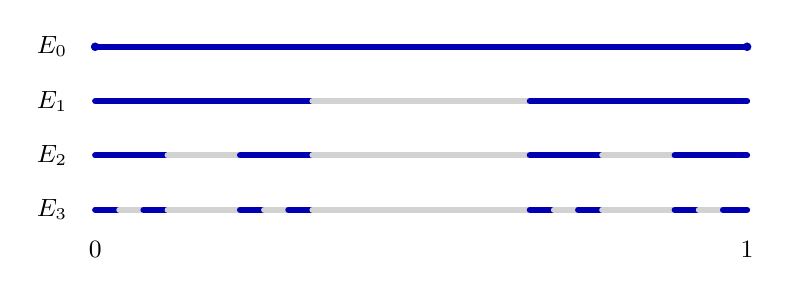
\begin{tikzpicture}[
  every node/.style={font=\small},
  stage/.style={blue!70!black, line width=2.2pt, line cap=round},
  gap/.style={gray!35, line width=2.2pt, line cap=round},
  endpoint/.style={circle, fill=blue!70!black, inner sep=1.1pt},
  scale=0.92
]
  \node[anchor=east] at (-0.25,0) {$E_0$};
  \draw[stage] (0,0) -- (9,0);

  \node[anchor=east] at (-0.25,-0.75) {$E_1$};
  \draw[stage] (0,-0.75) -- (3,-0.75);
  \draw[gap] (3,-0.75) -- (6,-0.75);
  \draw[stage] (6,-0.75) -- (9,-0.75);

  \node[anchor=east] at (-0.25,-1.5) {$E_2$};
  \draw[stage] (0,-1.5) -- (1,-1.5);
  \draw[gap] (1,-1.5) -- (2,-1.5);
  \draw[stage] (2,-1.5) -- (3,-1.5);
  \draw[gap] (3,-1.5) -- (6,-1.5);
  \draw[stage] (6,-1.5) -- (7,-1.5);
  \draw[gap] (7,-1.5) -- (8,-1.5);
  \draw[stage] (8,-1.5) -- (9,-1.5);

  \node[anchor=east] at (-0.25,-2.25) {$E_3$};
  \draw[stage] (0,-2.25) -- (1/3,-2.25);
  \draw[gap] (1/3,-2.25) -- (2/3,-2.25);
  \draw[stage] (2/3,-2.25) -- (1,-2.25);
  \draw[gap] (1,-2.25) -- (2,-2.25);
  \draw[stage] (2,-2.25) -- (7/3,-2.25);
  \draw[gap] (7/3,-2.25) -- (8/3,-2.25);
  \draw[stage] (8/3,-2.25) -- (3,-2.25);
  \draw[gap] (3,-2.25) -- (6,-2.25);
  \draw[stage] (6,-2.25) -- (19/3,-2.25);
  \draw[gap] (19/3,-2.25) -- (20/3,-2.25);
  \draw[stage] (20/3,-2.25) -- (7,-2.25);
  \draw[gap] (7,-2.25) -- (8,-2.25);
  \draw[stage] (8,-2.25) -- (25/3,-2.25);
  \draw[gap] (25/3,-2.25) -- (26/3,-2.25);
  \draw[stage] (26/3,-2.25) -- (9,-2.25);

  \foreach \x in {0,9} {
    \node[endpoint] at (\x,0) {};
  }
  \node[below] at (0,-2.55) {$0$};
  \node[below] at (9,-2.55) {$1$};
\end{tikzpicture}

  \caption{The retained intervals shrink from $E_0$ through $E_3$, while the middle-third gaps persist.}
  \label{fig:cantor-set-first-stages}
\end{illustrationfigure}

\begin{proposition} \label{prop:cantor-set-basic-topological-properties} \hlt{Basic Topological Properties of the Cantor Set}\\
Let $(\mathcal{I}_n)_{n\in\N_0}$, $(E_n)_{n\in\N_0}$, and $P$ be as in Definition \ref{def:cantor-set}.
\begin{enumerate}[label=(\roman*)]
\setlength{\itemsep}{0pt}
\item $(\forall n\in\N_0)$, the family $\mathcal{I}_n$ consists of $2^n$ pairwise disjoint compact intervals of length $3^{-n}$.
\item $(\forall n\in\N_0)\,E_{n+1}\subseteq E_n$.
\item The set $P$ is nonempty and compact.
\item The set $P$ contains no interval with two distinct points.
\item The set $P$ is perfect.
\end{enumerate}
\begin{proof}
\begin{enumerate}[label=(\roman*)]
\setlength{\itemsep}{0pt}
\item For $m\in\N$, let $Q_m$ denote claim (i) at $n=m-1$. The statement $Q_1$ holds by $\mathcal{I}_0=\{[0,1]\}$.\\
Under $Q_m$, each $[a,b]\in\mathcal{I}_{m-1}$ has two disjoint compact children in $\mathcal{I}_m$, each of length $\frac{b-a}{3}=3^{-m}$.\\
Children of distinct parents are disjoint, so $\#\mathcal{I}_m=2\cdot2^{m-1}=2^m$ and $Q_m\Rightarrow Q_{m+1}$.\\
Therefore $(\forall m\in\N)\,Q_m$ by Theorem \ref{thm:mathematical-induction}, which establishes (i).
\item $(\forall n\in\N_0)\,E_{n+1}\subseteq E_n$ by Definition \ref{def:cantor-set}.
\item Fix $n\in\N_0$. The set $E_n$ is nonempty by (i) and Definition \ref{def:cantor-set}. Each $I\in\mathcal{I}_n$ is closed by (i) and Theorem \ref{thm:compact-subsets-of-metric-spaces-closed}.\\
Hence $E_n$ is closed by Theorem \ref{thm:metric-open-closed-set-calculus}(iv). The inclusion $E_n\subseteq E_0=[0,1]$ holds by (ii), so $E_n$ is bounded.\\
Hence $E_n$ is compact by Theorem \ref{thm:heine-borel-rk}, direction $(i)\Rightarrow(ii)$. Since $E_1\subseteq E_0$, $P=\bigcap\limits_{n=1}^{\infty}E_n\neq\emptyset$ by Corollary \ref{cor:nested-nonempty-compact-intersection}.\\
The set $P$ is closed by Theorem \ref{thm:metric-open-closed-set-calculus}(ii). Since $P\subseteq E_0$ and $E_0$ is compact, $P$ is compact by Theorem \ref{thm:closed-subsets-of-compact-sets-compact}.
\item Suppose $J\subseteq P$ is an interval containing $u<v$. Choose $n\in\N$ with $3^{-n}<v-u$ by Theorem \ref{thm:special-sequence-limits}(v) with $x=\frac13$.\\
Choose $I_u,I_v\in\mathcal{I}_n$ with $u\in I_u$ and $v\in I_v$ by Definition \ref{def:cantor-set}. Intervals $I_u$ and $I_v$ are distinct by (i), $3^{-n}<v-u$.\\
Order $\mathcal{I}_n$ from left to right; then $I_u$ precedes $I_v$ by $u<v$. (i). Choose adjacent $[a,b],[c,d]$ in block from $I_u$ to $I_v$ with $b<c$.\\
Then $w\defeq\frac{b+c}{2}\in(u,v)\setminus E_n$. But $w\in J\subseteq P\subseteq E_n$ by Definition \ref{def:euclidean-intervals-cells-balls-convex}(ii), a contradiction.
\item Fix $x\in P$ and $\varepsilon>0$. Choose $n\in\N$ with $3^{-n}<\varepsilon$ by Theorem \ref{thm:special-sequence-limits}(v) with $x=\frac13$.\\
The point $x$ lies in a unique $I_n(x)\in\mathcal{I}_n$ by (i) and Definition \ref{def:cantor-set}. Choose an endpoint $y\neq x$ of $I_n(x)$.\\
One has $(\forall m\in\N_0)\,[m\leq n\Rightarrow y\in E_m]$ by (ii). Each parent endpoint remains in one child by Definition \ref{def:cantor-set}.\\
Hence $(\forall m\in\N_0)\,[m\geq n\Rightarrow y\in E_m]$ by Theorem \ref{thm:mathematical-induction} with index shift $j=m-n+1$.\\
Thus $y\in P$ and $0<\abs{x-y}\leq3^{-n}<\varepsilon$ by (i). Hence $x\in P^{\operatorname{acc}}$ by Definition \ref{def:metric-topology-core-definitions}(v).\\
The set $P$ is closed by (iii) and Theorem \ref{thm:compact-subsets-of-metric-spaces-closed}. Hence $P$ is perfect by Definition \ref{def:bounded-and-perfect-metric-sets}(ii).
\end{enumerate}
\hlt{Structural Commentary}: Induction establishes stage geometry; nested compactness and endpoint persistence control the limit.\\
\hlt{Key Insight}: Each stage shrinks components while preserving endpoints and opening gaps.
\end{proof}
\end{proposition}
